\documentclass[twocolumn,traditabstract]{aa}  

\usepackage{amsmath}
\usepackage{fixltx2e}
\usepackage[english]{babel}
\usepackage{graphicx}
\usepackage{epstopdf}
\usepackage{epsf,color}
\usepackage[mathscr]{eucal}
\usepackage{amsmath}
\usepackage{amssymb,amsfonts}
\usepackage{natbib}
\usepackage{graphicx}
\usepackage{txfonts}
\usepackage{dsfont}
\definecolor{Mygreen}{rgb}{0.75, 0.0, 0.0}
\definecolor{Mypink}{rgb}{1.0, 0.0, 0.5}
\definecolor{Myred}{rgb}{0.7, 0.0, 0.0}
\usepackage[breaklinks, citecolor=blue, linkcolor=Myred, urlcolor=Myred, colorlinks=true, debug, baseurl=' ']{hyperref}
\usepackage{float} 
\usepackage{color}

\bibpunct{(}{)}{;}{a}{}{,}
\bibliographystyle{aa}

\newfont{\gwpfont}{cmssq8 scaled 1000}
\newcommand{\rexcess}{{\gwpfont REXCESS}}
%%%%%%%%%%%%%%%%%%%%%%%%%%%%%%%%%%%%%%%%%%%%%%%%%%%%%%%%%%%%%%%%%%%%%%%%%
%\documentclass[iop,numberedappendix,apj]{emulateapj}
%\documentclass[iop,numberedappendix,apj]{aastex}
%\documentclass{article}
%\usepackage{emulateapj}
%\pdfoutput=1
%\usepackage{color}
%\usepackage{amssymb}
%\PassOptionsToPackage{hyphens}{url}
%\usepackage{hyperref}
%\usepackage{breakurl}
%\def\UrlBreaks{\do\/\do-}
%\usepackage{natbib}
%\usepackage{graphicx}
%\usepackage{epsfig}
%\usepackage[hyphens]{url}
%\usepackage{csquotes}
%\usepackage{lscape}
%\usepackage{afterpage}
%\usepackage[tbtags]{amsmath}
%\usepackage{hyperref,xcolor}
%\hypersetup{colorlinks,linkcolor={blue!50!black},citecolor={blue!50!black},urlcolor={blue!80!black}}
%\setlength{\tabcolsep}{0.04in} 
%\usepackage{epsfig}
%\usepackage{fullpage}
%\usepackage{hyperref}
%%%%%%%%%%%%%%%%%%%%%%%%%%%%%%%%%%%%%%%%%%%%%%%%%%%%%%%%%%%%%%%%%%%%%%%%%%%%%%%
%%% NOTES ON COMPILING / PRINTING THIS DOCUMENT
%%% do the latex <filename>
%%% dvips -O 0cm,2.0cm <filename.dvi>
%%% dvips -O 0cm,2.0cm clash_pressures.dvi

\newcommand {\apgt} {\ {\raise-.5ex\hbox{$\buildrel>\over\sim$}}\ }
\newcommand {\aplt} {\ {\raise-.5ex\hbox{$\buildrel<\over\sim$}}\ }
\newcommand{\dmod}{\overrightarrow{d}_{mod}}
\newcommand{\dvec}{\overrightarrow{d}}
\newcommand{\avec}{\overrightarrow{a}}
\newcommand{\asec}{$^{\prime \prime}$}
\newcommand{\asecs}{$^{\prime \prime}\ $}
\newcommand{\amin}{$^{\prime}$}
\newcommand{\amins}{$^{\prime}\ $}
\newcommand{\sigT}{\mbox{$\sigma_{\mbox{\tiny T}}$}}
\newcommand{\Tcmb}{\mbox{$T_{\mbox{\tiny CMB}}$}}
\newcommand{\kB}{\mbox{$k_{\mbox{\tiny B}}$}}
\newcommand{\kBT}{\mbox{$k_{\mbox{\tiny B}}T_{\mbox{\tiny e}}$}}
\newcommand{\nH}{\mbox{$n_{\mbox{\tiny H}}$}}
\newcommand{\NH}{\mbox{$N_{\mbox{\tiny H}}$}}
\newcommand{\LameH}{\mbox{$\Lambda_{e \mbox{\tiny H}}$}}
\newcommand{\Lamee}{\mbox{$\Lambda_{ee}$}}
\newcommand{\rhogas}{\mbox{$\rho_{\mbox{\scriptsize gas}}$}}
\newcommand{\rhotot}{\mbox{$\rho_{\mbox{\scriptsize tot}}$}}
\newcommand{\Mgas}{\mbox{$M_{\mbox{\scriptsize gas}}$}}
\newcommand{\Mtot}{\mbox{$M_{\mbox{\scriptsize tot}}$}}
\newcommand{\Mvir}{\mbox{$M_{\mbox{\scriptsize vir}}$}}
\newcommand{\Yint}{\mbox{$Y_{\mbox{\scriptsize int}}$}}
\newcommand{\Ycyl}{\mbox{$Y_{\mbox{\scriptsize cyl}}$}}
\newcommand{\Ysph}{\mbox{$Y_{\mbox{\scriptsize sph}}$}}
\newcommand{\fgas}{\mbox{$f_{\mbox{\scriptsize gas}}$}}
\newcommand{\LCDM}{\mbox{$\Lambda$CDM}}
\newcommand{\Pe}{\mbox{$P_{\mbox{\scriptsize e}}$}}
\newcommand{\msun}{$M_{\odot}$}
\newcommand{\etal}{{\it et al.}}
\newcommand{\mJy}{\,{\rm mJy} }
\newcommand{\um}{\,\mu {\rm m} }
\newcommand{\mJySr}{\,{\rm MJy/Sr} }
\newcommand{\mJyBm}{\,{\rm mJy/Bm} }
\newcommand{\mK}{\,{\rm mK} }
\newcommand{\K}{\,{\rm K} }
\newcommand{\uJy}{\,{\rm \mu Jy} }
\newcommand{\uK}{\,{\rm \mu K} }
\newcommand{\kHz}{\, {\rm kHz} }
\newcommand{\eg}{{\it e.g.}}
\newcommand{\ie}{{\it i.e.}}
\newcommand{\etc}{{\it etc.}}
\newcommand{\aips}{{\tt AIPS++}}
\newcommand{\nusp}{\nu_{sp}}
\newcommand{\ghz}{{\, \rm GHz}}
\newcommand{\db}{{\, \rm dB}}
\newcommand{\degsqr}{\, {\rm deg^2}}
\newcommand{\Tew}{\mbox{$T_{\mathrm{ew}}$}}
\newcommand{\Tspec}{\mbox{$T_{\mathrm{spec}}$}}
\newcommand{\chandra}{{\it Chandra}}
\newcommand{\asca}{{ASCA}}
\newcommand{\wmap}{{WMAP}}
\newcommand{\rosat}{{ROSAT}}
\newcommand{\xmm}{{XMM-{\it Newton}}}
\newcommand{\planck}{{\it Planck}}
\newcommand{\hubble}{{\it Hubble}}
\newcommand{\rxj}{RX J1347.5-1145}
\newcommand{\clj}{CL J1226.9+3332}
\newcommand{\macsa}{MACS J0647.7+7015}
\newcommand{\macsb}{MACS J1206.2-0847}
\newcommand{\macsc}{MACS J0717.5+3745}
\newcommand{\macsd}{MACS J1423.8+2404}
\newcommand{\macse}{MACS J0329.6-0211}
\newcommand{\macsf}{MACS J0429-0253}
\newcommand{\macsg}{MACS J0744.9+3927}
\newcommand{\macsh}{MACS J1149+2223}
\newcommand{\macsi}{MACS J1115+0130}
\newcommand{\Tx}{\mbox{$T_{\mbox{\tiny X}}$}}
\newcommand{\te}{\mbox{$T_{\mbox{\tiny e}}$}}
\newcommand{\mec}{\mbox{$m_{\mbox{\tiny e}} c^2$}}
\newcommand{\dene}{\mbox{$n_{\mbox{\tiny e}}$}}
\newcommand{\denesq}{\mbox{$n^2_{\mbox{\tiny e}}$}}
\newcommand{\yx}{\mbox{$Y_{\mbox{\tiny X}}$}}
\newcommand{\ysze}{\mbox{$Y_{\mbox{\tiny tSZE}}$}}
\newcommand{\sx}{\mbox{$S_{\mbox{\tiny X}}$}}
\newcommand{\Itsz}{\mbox{$I_{\mbox{\tiny tSZE}}$}}
\newcommand{\Iksz}{\mbox{$I_{\mbox{\tiny kSZE}}$}}
\newcommand{\chisq}{\mbox{$\chi^{2}$}}
\newcommand{\chired}{\mbox{$\chi^{2}_{red}$}}

\defcitealias{arnaud2010}{A10}
\defcitealias{cavagnolo2009}{C09}
\defcitealias{bulbul2010}{B10}
\defcitealias{vikhlinin2006a}{V06}

\newcommand{\quotes}[1]{``#1''}

%\slugcomment{}
%\shortauthors{Romero \etal}
%\shorttitle{Joint SZE Map Fitting with MUSTANG and Bolocam}
%altaffilmark{#}

\begin{document}

\title{Joint Fitting of CLJ1226.9}
\author{C.~Romero\inst{\ref{inst1}} \thanks{Corresponding author: Charles Romero, \url{romero@iram.fr}}			        %CT
\and M.~McWilliam\inst{\ref{inst2}}
\and R.~Adam\inst{\ref{inst3}}	                        %CT
\and P.~Ade\inst{\ref{inst4}}				%CT
\and P.~Andr\'e\inst{\ref{inst4}}			%CT
\and M.~Arnaud\inst{\ref{inst5}}
\and I.~Bartalucci\inst{\ref{inst4}}
\and A.~Beelen\inst{\ref{inst6}}			%CT
\and A.~Beno\^it\inst{\ref{inst7}}			%CT
\and A.~Bideaud\inst{\ref{inst4}}			%CT
\and N.~Billot\inst{\ref{inst8}}			%CT
\and H.~Bourdin\inst{\ref{inst9}}
\and O.~Bourrion\inst{\ref{inst10}}			%CT
\and M.~Calvo\inst{\ref{inst7}}				%CT
\and A.~Catalano\inst{\ref{inst10}}			%CT
\and G.~Coiffard\inst{\ref{inst1}}			%CT
\and B.~Comis\inst{\ref{inst10}}				%CT
\and F.-X.~D\'esert\inst{\ref{inst12}}			%CT
\and S.~Doyle\inst{\ref{inst4}}				%CT
\and C.~Ferrari\inst{\ref{inst1}}
\and J.~Goupy\inst{\ref{inst7}}				%CT
\and O.~Hahn\inst{\ref{inst1}}
\and C.~Kramer\inst{\ref{inst8}}			%CT
\and G.~Lagache\inst{\ref{inst13}}
\and S.~Leclercq\inst{\ref{inst1}}			%CT
\and J.-F.~Mac\'ias-P\'erez\inst{\ref{inst10}}	        %CT
\and S.~Maurogordato\inst{\ref{inst1}}
\and P.~Mauskopf\inst{\ref{inst4}, \ref{inst14}}	%CT
\and F.~Mayet\inst{\ref{inst10}}				%CT
\and A.~Monfardini\inst{\ref{inst7}}			%CT
\and F.~Pajot\inst{\ref{inst6}}				%CT
\and E.~Pascale\inst{\ref{inst4}}			%CT
\and L.~Perotto\inst{\ref{inst10}}			%CT
\and G.~Pisano\inst{\ref{inst4}}			%CT
\and E.~Pointecouteau\inst{\ref{inst16}, \ref{inst17}}
\and N.~Ponthieu\inst{\ref{inst12}}			%CT
\and G.W.~Pratt\inst{\ref{inst4}}
\and V.~Rev\'eret\inst{\ref{inst4}}			%CT
\and A.~Ritacco\inst{\ref{inst10}}			%CT
\and L.~Rodriguez\inst{\ref{inst4}}			%CT
\and F.~Ruppin\inst{\ref{inst10}}			%CT
\and K.~Schuster\inst{\ref{inst1}}			%CT
\and A.~Sievers\inst{\ref{inst8}}			%CT
\and S.~Triqueneaux\inst{\ref{inst7}}		        %CT
\and C.~Tucker\inst{\ref{inst4}}			%CT
\and R.~Zylka\inst{\ref{inst1}}}			%CT

\institute{
Institut de RadioAstronomie Millim\'etrique (IRAM), Grenoble, France
  \label{inst1}
  \and
Imperial College London, Kensington, London SW7 2AZ, UK
  \label{inst2}
  \and
Laboratoire Lagrange, Universit\'e C\^ote d'Azur, Observatoire de la C\^ote d'Azur, CNRS, Blvd de l'Observatoire, CS 34229, 06304 Nice cedex 4, France
  \label{inst3}
  \and
Astronomy Instrumentation Group, University of Cardiff, UK
  \label{inst4}
  \and
Laboratoire AIM, CEA/IRFU, CNRS/INSU, Universit\'e Paris Diderot, CEA-Saclay, 91191 Gif-Sur-Yvette, France 
  \label{inst5}
  \and
Institut d'Astrophysique Spatiale (IAS), CNRS and Universit\'e Paris Sud, Orsay, France
  \label{inst6}
  \and
Institut N\'eel, CNRS and Universit\'e Grenoble Alpes, France
  \label{inst7}
  \and
Institut de RadioAstronomie Millim\'etrique (IRAM), Granada, Spain
  \label{inst8}
  \and
Dipartimento di Fisica, Universit\`a degli Studi di Roma 'Tor Vergata', via della Ricerca Scientifica, 1, I-00133 Roma, Italy
  \label{inst9}
  \and
Laboratoire de Physique Subatomique et de Cosmologie, Universit\'e Grenoble Alpes, CNRS/IN2P3, 53, avenue des Martyrs, Grenoble, France
  \label{inst10}
  \and
Dipartimento di Fisica, Sapienza Universit\`a di Roma, Piazzale Aldo Moro 5, I-00185 Roma, Italy
  \label{inst11}
  \and
Institut de Plan\'etologie et d'Astrophysique de Grenoble (IPAG), CNRS and Universit\'e Grenoble Alpes, France
  \label{inst12}
  \and
Aix Marseille Universit\'e, CNRS, LAM (Laboratoire d'Astrophysique de Marseille) UMR 7326, 13388, Marseille, France
  \label{inst13}
  \and
School of Earth and Space Exploration and Department of Physics, Arizona State University, Tempe, AZ 85287
  \label{inst14}
  \and
Universit\'e de Toulouse, UPS-OMP, Institut de Recherche en Astrophysique et Plan\'etologie (IRAP), Toulouse, France
  \label{inst16}
\and
CNRS, IRAP, 9 Av. colonel Roche, BP 44346, F-31028 Toulouse cedex 4, France 
  \label{inst17}
}

%%%%%%%%%%%%%%%%%%%%%%%%
%\author{
%  Order TBD ,
%  Charles E. Romero\altaffilmark{1,*},
%  Matthew McWilliam \altaffilmark{2,3},
%  Juan Macias-Perez \altaffilmark{3},
%  NIKA Collaboration \altaffilmark{4}
%} 
%\date{\today}
\date{Received \today \ / Accepted --}

%%%%%%%%%%%%%%%%%%%%%%%%%%%%%%%%%%%%%%%%%%%%%%%%%%%%%%%%%%%%%%%%%%%%%%%%%%%%%%%
%\altaffiltext{1}{Institut de Radioastronomie Millim\'{e}trique
%300 rue de la Piscine, Domaine Universitaire
%38406 Saint Martin d'H\`{e}res, France} 
%\altaffiltext{2}{Imperial College London, Kensington, London SW7 2AZ, UK}
%\altaffiltext{3}{Laboratoire de Physique Subatomique et Cosmologie 53 Avenue des Martyrs, 38000 Grenoble}
%\altaffiltext{4}{NIKA2 Collaboration}
%\altaffiltext{*}{Author contact: \email{romero@iram.fr}}
%\begin{document}

%%%%%%%%%%%%%%%%%%%%%%%%%%%%%%%%%%%%%%%%%%%%%%%%%%%%%%%%%%%%%%%%%%%%%%%%%%%%%%%

%\begin{abstract}
\abstract
    {We present non-parametric pressure profiles of a galaxy cluster, CLJ 1226.9+3352, as
      determined from SZ data from the MUSTANG, NIKA, and Bolocam instruments.
      We note that, despite the differences in angular resolution,
      observing frequency, and observing strategies, there is generally good agreement.
      Given that for a given instrument, constraints on the pressure profile
      diminish rapidly beyond the field of view, the overlap in spatial sensitivity
      of these three datasets is critical in checking for consistency between instruments,
      and in the process provides continuous coverage over the radial scales
      $0.05 R_{500} < r < 2 R_{500}$. Despite this coverage, with these instruments alone, we
      still suffer from poor constraints at the largest radii, and therefore include a prior
      from Planck on the integrated Compton Y parameter. Our non-parametric algorithm makes
      use of logarithmic interpolation, which under the assumption of ellisoidal symmetry is
      analytically integrable.}
%\end{abstract}

\titlerunning{Non-parametric fitting with MUSTANG, NIKA, Bolocam, and Planck}
\authorrunning{C. Romero, M. McWilliam, and the NIKA SZ team}
\keywords{-- Galaxies: clusters: individual: CLJ1226.9+3352}

\maketitle

%%%%%%%%%%%%%%%%%%%%%%%%%%%%%%%%%%%%%%%%%%%%%%%%%%%%%%%%%%%%%%%%%%%%%%%%%%%%%%%
\section{Introduction}
\label{sec:intro}
%%%%%%%%%%%%%%%%%%%%%%%%%%%%%%%%%%%%%%%%%%%%%%%%%%%%%%%%%%%%%%%%%%%%%%%%%%%%%%%

%\textcolor{red}{Edit author list - add in Matthew McWilliam (again).}

In recent years, Sunyaev Zel'dovich (SZ) effect observations have seen an increase in high resolution ($\theta \lesssim 30$\asecs)
observations \citep[e.g.][]{mason2010,adam2014,kitayama2016}. These observations come from MUSTANG on the
Robert C. Byrd Green Bank Telescope \citep[GBT][]{dicker2008}, NIKA on the IRAM 30-meter telescope \citep{monfardini2010},
and ALMA, band 3 observations. However, all of these high resolution instruments have been limited in their ability to
recover signal at large scales (beyond $\sim 45$'asecs for MUSTANG and ALMA, and $\sim 100$\asecs for NIKA). As galaxy clusters
have characteristic radii, $R_{500} \gtrsim 3$\amin, SZ observations made with these instruments have not been able to recover the
entire signal of the observed galaxy clusters. Therefore, observations from SZ instruments which recover SZ at larger scales
such as Bolocam \citet{czakon2015} or Planck \citep{planck2013a} have been used in \citet{romero2015a} and \citet{adam2014} respectively.

These joint analyses have shown the ability to constrain the pressure profile of the intracluster medium (ICM) of individual
galaxy clusters over a large spatial range, often by assuming some parameterized pressure profile \citep[e.g.][]{romero2016,adam2014}.
In \citet{romero2015a}, the difference in fitted pressure profiles with the addition of MUSTANG data was noted. In the case of
\citet{romero2016,adam2014}, the pairs of instruments used did not have an overlap in scales of instrument sensitivity, so the
addition of another instrument would not necessarily present any discrepancies. However, as new SZ instruments with sensitivity to
a larger range of scales come online \citep{monfardini2014,dicker2014a}, there will be overlap, which for clusters observed with
multiple instruments, studies of the kinetic SZ effect, or relativistic corrections \citep{itoh1998} will be of significant interest and
stand to benefit from the additional frequency coverage. To be sure of the results of these analyses, it will be critical to
understand any systematics involved with individual instruments. Recent results combining Bolocam and Planck data \citep{sayers2016},
which overlap in regions of sensitivity, show non-trivial changes from previous Bolocam-only results \citep{sayers2013}.

Many SZ analyses thus far have focused on fitting a smooth pressure profile to their data; over a decade ago, the beta model
\citep{cavaliere1978} was used. While a self-similar \citep{mroczkowski2009} and analytical pressure profile based on a
polytropic equation of state \citep{bulbul2010} have been explored, the general Navaro-Frenk-and-White
\citep[gNFW][]{nagai2007} has garnered the most traction, with a fairly canonical set of parameters coming from
\citet{arnaud2010} (Hereafter, A10). While some SZ studies have attempted to deproject their data \citep[e.g.][]{sayers2013},
and fit pressure profiles to their deprojected data, the publication of non parametric pressure profile constraints have
been scarce. Investigating cluster pressure profiles non parametrically will show deviations from the smooth pressure profile,
which could be cause either due to systematics or inherent physical pertubations. That is, if we wish to better understand
discrepancies between SZ constraints, as discussed previously, investigating the non-parametric fits between instruments will
provide a viable route to this end. Independently, understanding pertubations within the cluster itself is also important in
the context of using galaxy clusters as cosmological probes.

Counts of galaxy clusters by mass and redshift serve to constrain cosmological parameters, notably $\Omega_{\Lambda}$,
the amplitude of fluctuations, $\sigma_8$, and the equation of state of dark energy, $w$. Constraints on these
parameters derived from galaxy cluster samples are generally limited by the accuracy of mass estimation of 
galaxy clusters \citep[e.g.][]{hasselfield2013, reichardt2013}. Scaling relations which relate global (integrated) observables
to the cluster mass are often employed. Currently, scaling relations as applied to observables over an intermediate radial
region of galaxy clusters is preferred as this range shows minimal scatter in the scaling relations \citep[e.g.][]{kravtsov2012}
owing to the generally low cluster-to-cluster scatter in pressure profiles, found observationally and in simulations,
within this radial range \citep[e.g.][]{borgani2004,nagai2007,arnaud2010,bonamente2012,planck2013a,sayers2013}.
While the relative homogeneity of pressure profiles in the intermediate region is well evidenced, it remains important to
develop methods to derive non-parametric pressure profiles of clusters so that physical deviations are not artificially
smoothed by the adoption of a smooth parametric profile. 

This paper is organized as follows. In Section~\ref{sec:obs} we review the NIKA, MUSTANG, and Bolocam observations and reduction. 
In Section~\ref{sec:ml_deproj} we address the method used to non-parametrically fit pressure profiles to each of the data sets.
%We present results from the joint fits in Section~\ref{sec:pp_constraints} and compare our results to X-ray derived pressures 
%in Section~\ref{sec:xray_comp}. 
Throughout this paper we assume a $\Lambda$CDM cosmology with $\Omega_m = 0.28$, $\Omega_{\lambda} = 0.72$, and $H_0 = 70$ 
km s$^{-1}$ Mpc$^{-1}$, consistent with the 9-year \emph{Wilkinson Microwave Anisotropy Probe} (WMAP) results reported
in \cite{hinshaw2013}.

%%%%%%%%%%%%%%%%%%%%%%%%%%%%%%%%%%%%%%%%%%%%%%%%%%%%%%%%%%%%%%%%%%%%%%%%%%%%%%%
\section{Observations and Data Reduction}
\label{sec:obs}
%%%%%%%%%%%%%%%%%%%%%%%%%%%%%%%%%%%%%%%%%%%%%%%%%%%%%%%%%%%%%%%%%%%%%%%%%%%%%%%

\subsection{CLJ1226.9+3352}
\label{sec:sample_clj1227}

%%%%%%%%%%%%%%%%%%%%%%%%%%%%%%%%%%%%%%%%%%%%%%%%%%%%%%%%%%%%%%

% \textcolor{red}{I have to reword this subsection.}

At a redshift of $z=0.89$, CLJ1226.9+3352, hereafter CLJ 1227, is a massive cluster which was first discovered in the
Wide Angle ROSAT Pointed Survey \citep[WARPS][]{ebeling2001}. It has succesively been well studied
in the X-ray
\citep[\emph{XMM},\emph{Chandra}, and \emph{XMM/Chandra}][, respectively]{maughan2004,bonamente2006,maughan2007}
and SZ \citep[][]{joy2001,muchovej2007,mroczkowski2009,mroczkowski2011,bulbul2010,korngut2011,adam2015}.
In \citet{maughan2007}, the identification of hot southwestern component gave the first indications of disturbance
in this cluster. This interpretation was further bolstered by HST observations \citep{jee2009}, in which the lensing
analysis revealed two distinct peaks, one of which was coincident with the hot X-ray temperature region.

Given the relative circular symmetry of CLJ 1227, it provides a suitable test for determining a non-parametric pressure
profile of the cluster, while maintaining the assumption of spherical symmetry. For the centroid, we adopt the X-ray
centroid from ACCEPT \citep{cavagnolo2009} is at [RA,Dec] = [12:26:57.9,+33:32:49] (J2000).
From X-ray data, \citet{mantz2010} find a scale radius $R_{500} = 1000$ kpc, which corresponds to
$M_{500} = 12.0 \times 10^{14} M_{\odot}$.

\begin{figure*}[!h]
  \centering
%  \includegraphics[width=0.5\textwidth]{NIKA_ml_deproj_figs/CLJ1227_MUSTANG_NIKA_Bolocam_v2.eps}
  \includegraphics[width=0.33\textwidth]{NIKA_ml_deproj_figs/MUSTANG_image_and_SNR_contours_v2.eps}
  \includegraphics[width=0.33\textwidth]{NIKA_ml_deproj_figs/NIKA_image_and_SNR_contours_v2.eps}
  \includegraphics[width=0.33\textwidth]{NIKA_ml_deproj_figs/BOLOCAM_image_and_SNR_contours_v2.eps}
  \caption{Left: MUSTANG map; Middle: NIKA (2mm) map; Right: Bolocam map. In all three panels, the yellow contours are those
    of MUSTANG, magenta contours of those of NIKA, and cyan contours are those of Bolocam. For MUSTANG and Bolocam, the contours
    start at $(-)2\sigma$, with $1\sigma$ increments. For NIKA, the contours start at $(-)3\sigma$ with $2\sigma$ increments.
    The point source identified in \citet{adam2015} is subtracted in the MUSTANG
    and NIKA maps.}
  \label{fig:clj1227_maps}
\end{figure*}


%and a scaling pressure, $P_{500} = 11.7$keV/cm$^{3}$.

%%% K09 flux is 0.34 +/- 0.13 mJy in our maps. Now I've written it in. Jan 2016.

%\textcolor{red}{[I will do an analysis with the point source found in Korngut+2011. The question is if I already 
%have the point source modelled (and to find it).}

%\begin{deluxetable}{llllll}
%\tabletypesize{\footnotesize}
%\tablecolumns{10}
%\tablewidth{0pt} 
%\tablecaption{observational properties. \label{tbl:cluster_obs}}
%\tablehead{ 
%  \colhead{Instrument} & \colhead{Freq.} & \colhead{$T_{obs}$} & \colhead{Noise} &
%  \colhead{FWHM} & \colhead{FOV} \\
%  \colhead{ } & \colhead{(GHz)} & \colhead{(hours)} & \colhead{(Compton y)} &
%  \colhead{(\asec)} & \colhead{(\amin)}
%}
%\startdata
%\textbf{NIKA}    & 150 & 7.2  & $12.5 \times 10^{-6}$ & 18  & 1.9 \\
%\textbf{MUSTANG} &  90 & 4.9  & $34.2 \times 10^{-6}$ & 9   & 0.7 \\
%\textbf{Bolocam} & 150 & 11.8 & $8.48 \times 10^{-6}$ & 58  &   8 \\
%\textbf{Planck}  & 100 & ??   & ??                   & 588 & 5000 ? 
%\enddata
%\tablecomments{Overview of the sensitivities achieved for each of the instruments used in this analysis.}
%\end{deluxetable}

\begin{table*}[]
\caption{\footnotesize{Overview of the sensitivities achieved for each of the instruments used in this analysis.}}
\begin{center}
%\resizebox{\textwidth}{!} {
\begin{tabular}{l|lllll}
  \hline
  \hline
  Instrument & Freq. & $T_{obs}$ & Noise & FWHM & FOV \\
   & (GHz) & (hours) & (Compton y) & (\asec) & (\amin) \\
  \hline
  \textbf{NIKA}    & 150 & 7.2  & $12.5 \times 10^{-6}$ & 18  & 1.9 \\
  \textbf{MUSTANG} &  90 & 4.9  & $34.2 \times 10^{-6}$ & 9   & 0.7 \\
  \textbf{Bolocam} & 150 & 11.8 & $8.48 \times 10^{-6}$ & 58  &   8 \\
%  \textbf{Planck}  & 100 & ??   & ??                   & 588 & 5000 ? \\
  \hline
\end{tabular}
\end{center}
\label{tbl:cluster_obs}
\end{table*}


%%%%%%%%%%%%%%%%%%%%%%%%%%%%%%%%%%%%%%%%%%%%%%%%%%%%%%%%%%%%%%%%%%%%%%%%%%%%%%%
\subsection{NIKA Observations and Reduction}
\label{sec:nikaobs}
We use in this paper NIKA camera observations of the cluster CLJ 1227, which were obtained at the IRAM 30 m telescope (Pico Veleta) in February 2014 and presented in \citet{adam2015}. NIKA \citep{monfardini2010,monfardini2014} was a dual band camera working at 150 and 260 GHz, and made of 253 Kinetic Inductance Detectors (KIDs) operated at 100 mK by using a closed cycle $^3$He-$^4$He dilution fridge. 
Furthermore, with a sensitivity of 14 (35) mJy/beam.s$^{1/2}$ , a circular field-of-view (FOV) of 1.9$^{\prime}$ (1.8$^{\prime}$), and a resolution of 18.2$^{\prime \prime}$ (12.0$^{\prime \prime}$) at 150 (260) GHz NIKA was particularly well adapted to map the thermal Sunyaev-Zeldovich effect in such a high redshift cluster. NIKA conversion factors from mJy/beam to Compton parameter are $-10.9 \pm 0.8$ and $3.5\pm0.5$ at 150 and 260 GHz, respectively. A detailed description of the general performances of the camera can be found in \citet{catalano2014,adam2014}.

CLJ 1227 was mapped using on-the-fly raster scans made of 19 constant either azimuth, or elevation, subs-cans
of 6$^{\prime}$ length and separated by 10$^{\prime \prime}$. The observations were carried mainly by night with atmospheric opacities in the range 0.06-0.23 (0.06-0.29) at 150 (260) GHz. The overall on cluster effective time of observation was 7.8 hours. Pointing offsets were corrected during observations obtaining an overall pointing rms error below 3$^{\prime \prime}$. Uranus was used as a primary calibrator with overall calibration uncertainties of 7 \% and 12 \% at 150 and 260 GHz (respectively). The NIKA raw data was processed using the NIKA processing pipeline described in \citet{adam14} and \citet{adam15}. Low frequency atmospheric emission was removed using a common mode, which was computed iteratively after masking in the time domain the reconstructed cluster signal to a given signal-to-noise threshold. 
The processed data were projected into 2$^{\prime \prime}$ square pixels using inverse variance weighting and nearest grid projection.
The transfer function of the processing procedure was computed using signal plus noise simulations as described in \citet{adam2015}.
A full representation of the obtained transfer function is given in Figure 3 of \citet{adam2015} and it is used in this paper. Overall the transfer function is consistent with a constant value of 1 for angular scales scales smaller than the NIKA FOV and larger than the size of the NIKA beam. Using the 260~GHz NIKA map \citet{adam2015} identified a point source located 30$^{\prime \prime}$ southeast of the center of the cluster. The 150~GHz NIKA map, with the point source subtracted (Section~\ref{sec:preprocessing}) is shown in the middle panel
in Figure~\ref{fig:clj1227_maps}.

%%%%%%%%%%%%%%%%%%%%%%%%%%%%%%%%%%%%%%%%%%%%%%%%%%%%%%%%%%%%%%%%%%%%%%%%%%%%%%%
\subsection{MUSTANG Observations and Reduction}
\label{sec:musobs}
The MUSTANG camera \citep{dicker2008}
on the 100 meter Robert C. Byrd Green Bank Telescope \citep[GBT, ][]{jewell2004} with its angular resolution of 9\asec 
(full-width, half-maximum FWHM) is one of only a few SZ effect instruments with sub-arcminute resolution.
However, MUSTANG's instantaneous field of view (FOV) limits its sensitivity to scales larger than $1$\amin.
MUSTANG is a 64 pixel array of Transition Edge Sensor (TES) bolometers arranged in an $8 \times 8$ array
located at the Gregorian focus on the 100 m GBT. Operating at 90 GHz (81--99~GHz),
MUSTANG has an angular resolution of 9\asec and pixel spacing of 0.63$f \lambda$ resulting in a FOV
of 42\asec. More detailed information about the instrument can be found in \citet{dicker2008}.

Our observations and data reduction are described in detail in \citet{romero2015a}, and we briefly review them
here. Absolute flux calibrations are based on the planets Mars, Uranus, or Saturn, nebulae, or the star Betelgeuse 
($\alpha_{Ori}$). Responsive detectors are determined by scans taken at regular intervals with a calibration lamp.
We fit and subtract a common mode template, polynomial, and sinusoid. Further data quality checks are calculated
after this subtraction. The MUSTANG data map, with the point source subtracted (see Section~\ref{sec:preprocessing})
is shown in the left panel in Figure~\ref{fig:clj1227_maps}.


A transfer function was calculated in \citet{romero2016} when applied to white noise
across an entire sky. We find that said transfer function does not fully reproduce the results of a simulated
cluster observation. Therefore, we refine the the transfer function by filtering a cluster model based on a strictly
\citetalias{arnaud2010} profile (a gNFW profile with parameters
$[\alpha,\beta,\gamma,C_{500},P_0]=[1.05,5.49,0.31,1.18,8.42]$) through the standard MUSTANG pipeline and calculate
the transfer function. The principle difference between this new transfer function and the former transfer function
occurs at scales larger than the FOV (wavenumbers smaller than $\sim0.025$ inverse arcseconds).

%We verify the results of the transfer functions to the standard pipeline and find agreement,
%principally of the peak amplitude, within 10\%. To further
We verify the fidelity of the new transfer function by reproduce the analysis performed in \citet{romero2016} for CLJ1227,
with the use of the new transfer function in place of the standard MUSTANG filtering procedure.
In general, we find good agreement for the constraints on pressure profiles. More specifically, cluster models with
$0.5 < C_{500} < 3.3$ are well reproduced with fitted amplitudes that are within 10\% of those found in \citet{romero2016}.
Furthermore, the best fit profile shape parameters ($C_{500}$, $P_0$, and $\gamma$) are within $\sim10$\% agreement as well.


%%% How was the transfer function calculated 
%Maybe it just needs some words.\footnote{MUSTANG data is publicaly available at 
%\href{https://safe.nrao.edu/wiki/bin/view/GB/Pennarray/MUSTANG_CLASH}}

%%%%%%%%%%%%%%%%%%%%%%%%%%%%%%%%%%%%%%%%%%%%%%%%%%%%%%%%%%%%%%%%%%%%%%%%%%%%%%%
\subsection{Bolocam Observations and Reduction}
\label{sec:bolocamobs}

To probe a wider range of scales we complement our MUSTANG data with SZ data from Bolocam \citep{glenn1998}. 
Bolocam is a 144-element bolometer
array on the Caltech Submillimeter Observatory (CSO) with a beam FWHM of 58\asecs at 140 GHz and circular FOV with 8\amins 
diameter, which is well matched to the angular size of $R_{500}$ ($\sim 4$\amin) of the clusters in our sample. 

Bolocam is a 144-element camera that was a facility instrument on the Caltech Submillimeter Observatory (CSO) from
2003 until 2012. Its field of view is 8\amins in diameter, and at 140 GHz it has a resolution of 58\asecs FWHM
(\citet{glenn1998,haig2004}). The clusters were observed with a Lissajous pattern that results in a tapered
coverage dropping to 50\% of the peak value at a radius of roughly 5\amin, and to 0 at a radius of 10\amin.
The Bolocam maps used in this analysis are $14\arcmin \times 14\arcmin$. The Bolocam data 
%\footnote{Bolocam data is publicaly available at 
%\href{http://irsa.ipac.caltech.edu/data/Planck/release\_2/ancillary-data/bolocam/}
%{http://irsa.ipac.caltech.edu/data/Planck/release\_2/ancillary-data/} 
%\href{http://irsa.ipac.caltech.edu/data/Planck/release\_2/ancillary-data/bolocam/}{bolocam/}.} 
are the same as those used in \citet{czakon2015} and \citet{sayers2013}; the details of the reduction are 
given therein, along with \citet{sayers2011}. The (2mm) Bolocam map is shown in the right panel of Figure~\ref{fig:clj1227_maps}.
The reduction and calibration is similar to that used for MUSTANG, and Bolocam achieves a 
5\% calibration accuracy and 5\asecs pointing accuracy.

%%% How was the transfer function calculated 

\subsection{Planck integrated Compton parameter}
As in \citet{adam2015} we consider in the analysis the integrated Compton parameter of the cluster as measured using the Planck data.
We use the Planck frequency maps from 143 to 857~GHz to produce a Compton parameter map as described in \citet{hurier2013} and \citet{planck2013ymap,2016A&A...594A..22P}. The resolution of this map is 7.5$^{\prime}$, limited by the lowest frequency Planck channel map used in the reconstruction. Using this map we compute the integrated Compton parameter up to a radial distant of 15$^{\prime}$ with respect to the center of the cluster. Uncertainties in the integrated Compton parameter are computed by integrating at random positions around the cluster. The uncertainties obtained has been also crossed checked using Planck half-ring half difference Compton parameters obtained as described in \citet{planck2013ymap,2016A&A...594A..22P}. We find $Y_{15^{\prime}} = (0.94 \pm 0.36) \times 10^{-3}$ arcmin$^2$. 

%%%%%%%%%%%

%%%%%%%%%%%%%%%%%%%%%%%%%%%%%%%%%%%%%%%%%%%%%%%%%%%%%%%%%%%%%%%%%%%%%%%%%%%%%%%
\section{Pressure Profiles via Maximum Likelihood}
\label{sec:ml_deproj}
%%%%%%%%%%%%%%%%%%%%%%%%%%%%%%%%%%%%%%%%%%%%%%%%%%%%%%%%%%%%%%%%%%%%%%%%%%%%%%%

%\subsection{{\color{red}Overview}}
%\label{sec:ml_overview}

\subsection{Preprocessing}
\label{sec:preprocessing}

%PK location: [12:26:58.0,+33:32:59]

A point source at $4.6\sigma$ significance in MUSTANG was reported in \citet{korngut2011}, but is not
evident in the reprocessed MUSTANG data. A short VLA filler observation (VLA-12A-340, D-array, at 7 GHz) 
was performed to follow up this potential source (at RA 12:26:58.0 and Dec +33:32:59),
but to a limit of $\sim 50 {\rm \mu Jy}$ nothing is seen. At 500 $\mu$m, \emph{Herschel}-SPIRE has a
point source sensitivity of $\sim 8$ mJy, and therefore does not truly constrain a potential point
source at this location.

However, \citet{adam2015} find a point source at RA 12:27:00.01 and Dec +33:32:42 with a flux density of 
$6.8 \pm 0.7 \text{ (stat.)} \pm 1.0 \text{ (cal.)}$ mJy at 260 GHz and $1.9 \pm 0.2 \text{ (stat.)}$ at 150 GHz.
At 500 $\mu$m, \emph{Herschel}-SPIRE finds a flux of $100 \pm 8$ mJy.
\footnote{{http://irsa.ipac.caltech.edu/applications/Gator/}}
A point source at this location is fit to the MUSTANG data with a flux density of $0.36 \pm 0.11$ mJy
\citep{romero2016}. We subtract this point source from the NIKA and MUSTANG maps.

%A point source at $4.6\sigma$ significance in MUSTANG was reported in \citet{korngut2011}, but is not
%evident in the reprocessed MUSTANG data. A short VLA filler observation (VLA-12A-340, D-array, at 7 GHz) 
%was performed to follow up this potential source, but to a limit of $\sim 50 {\rm \mu Jy}$ nothing is seen.
%However, \citet{adam2015} find a point source at RA 12:27:00.01 and Dec +33:32:42 with a flux density of 
%$6.8 \pm 0.7 \text{ (stat.)} \pm 1.0 \text{ (cal.)}$ mJy at 260 GHz and $1.9 \pm 0.2 \text{ (stat.)}$ at 150 GHz. 
%A point source at this location is fit to the MUSTANG data with a flux density of $0.36 \pm 0.11$ mJy
%\citep{romero2016}. We subtract this point source from the NIKA and MUSTANG maps.

The mean level in the MUSTANG map is calculated as the mean within the inner arcminute MUSTANG noise map. 
We subtract the mean level from the MUSTANG map before fitting a cluster model. The Bolocam map already has
a mean level subtracted.  The point source is faint enough to not be a concern for the Bolocam data given
Bolocam's beam. No mean level is subtracted from NIKA.

\subsection{Non-Parametric Models}
\label{sec:np_models}

We employ a spherically symmetric pressure profile as our galaxy cluster model. Our fitting algorithm is applied
to each dataset independently; therefore, cluster models are binned and gridded differently for each dataset.
Radial bins are defined so that
each bin is at least as wide as a beam width, with the additional constraint that the outer most bin is beyond
the FOV of the instrument. We define our radial bins based on the radii which confine the bins. Our first bin
covers the range $0 < r < R_1$; our second bin covers $R_1 < r < R_2$, and our last ($n$th) bin covers
$R_{n-1} < r $, i.e. it extends to infinity. A finite radius $R_n$ is defined, and is used to determine the power
law in this outermost bin. Pressure normalizations, $P_i$, are defined at each bin boundary, $R_i$. We then assume
that the pressure in between bin boundaries follows a power law, $P \propto r^{-\alpha}$. We assume that the power
law in the first bin is given by the power law of the second bin.
The power law of the outermost bin is determined from $P_{n-1}$ (at $R_{n-1}$) and $P_{n}$ (at $R_{n}$), and extended
to infinity. Given the integration along the line of sight, we put a prior on this outer bin such that $\alpha > 1$.
We note that under hydrostatic equilibrium (HSE), this should be limited to $\alpha >3$ in order to avoid having
infinite mass.

Given the restrictions of ellptical symmetry and a power law dependence of the integrated quantity (pressure) on the
elliptical radius, it is possible to calculate the integral along the line of sight analytically
\citep[e.g.][]{vikhlinin2001a,korngut2011}. We follow
principally the formulation provided in \citet{korngut2011}. As noted in \citet{sarazin2016}, there are certain power
laws ($\alpha/2 = p = 1/2, 0 , -1/2, -1, -3/2, ...$) for which the formulation given in \citet{korngut2011} fails,
but a reformulation provides a valid integration. More generally, the formulation fails for $\alpha/2 = p < -1/2$.
While a negative index indicates a rise in pressure with radius (atypical), this could arise, especially localised,
from shocks, for example. We also wish to minimise our restrictions on the power laws (between bins) so as to minimise
induced correlations between bins. Therefore, we implement extensions to the canonical formuation that allow us to
integrate within finite regions (spheres or shells that extend only to a finite radius). These extensions and
reformulations of specific half integers and described in Section~\ref{sec:analytic_integrals}.

The integrated profiles, calculated as the Compton y parameter:
\begin{equation}
  y = \frac{\sigma_T}{m_e c^2} \int P_e dl,
  \label{eqn:compton_y}
\end{equation}
are converted into the units of the original data map. Maps are gridded by assuming a linear interpolation
of the 1D (radial) profiles.
When gridding our bulk ICM component, we adopt the ACCEPT centroid of CLJ 1227.
These maps are then convolved with the respective beam and transfer function.

%We do not find significant changes in
%the fitted gNFW parameters (Section~\ref{sec:pp_constraints}), 

\subsection{Fitting Algorithm}

%\textcolor{red}{I need to review emcee and Matt's write-up.}
We employ a maximum likelihood algorithm, and take our noise to be Gaussian such that our likelihood is given
by:
\begin{equation}
  \mathcal{L} \propto e^{-\chi^2 / 2} 
  \label{eqn:likelihood}
\end{equation}
and $\chi^2$ is given by:
\begin{equation}
  \chi^2 = (\overrightarrow{d} - \overrightarrow{d}_{mod})^T \mathbf{N}^{-1} (\overrightarrow{d} - \overrightarrow{d}_{mod}),
  \label{eqn:chi_sq}
\end{equation}
where $\overrightarrow{d}$ is our data, $\overrightarrow{d}_{mod}$ is our model, and $\mathbf{N}^{-1}$ is our
covariance matrix for a given dataset.

In previous works, NIKA and MUSTANG noise has been taken as uncorrelated \citep[e.g.][]{romero2015a,romero2016,adam2015}.
Bolocam noise has been taken as roughly uncorrelated, but 1000 noise realizations, which included CMB and point
source estimates, are provided to allow for a more accurate noise estimation \citep{sayers2011}.
%In \citet{romero2016},
%the 1000 Bolocam noise realizations were added to a best fit model (found assuming uncorrelated noise) to determine
%more appropriate constraints on fitted parameters.
We calculate the two-dimensional power spectrum for noise maps of each dataset and find that the noise is consistent
with white noise on the scales, for each dataset, which we wish to constrain the models.
%\textcolor{red}{Do we want a figure of these?}

We calculate the final probability of our models by applying priors as prescribed by Bayes' Theorem.
%\begin{equation}
%  P(\overrightarrow{d} | \theta) \propto \mathcal{L}(\theta | \overrightarrow{d}) \text{Prior}(\theta)
%  \label{eqn:prior}
%\end{equation}
On each of the pressure bins, we assign strict priors that $P_i > 0$, and as previously mentioned, the last bin
has a prior that on its associated power law slope: $\alpha > 1$. We allow for the choice of including a prior
on the integrated Compton Y parameter:
\begin{equation}
  Y = \int y d\Omega,
  \label{eqn:integrated_y}
\end{equation}
where the integral over solid angle taken within a given radius is generally referred to as the cylindrical
Compton Y value ($Y_{cyl}$). We calculate $Y_{cyl}$ using the un-filtered Compton y profile (before convolution with
an instrument's beam and transfer function). The prior on Y comes
%\textcolor{red}{(Need to introduce this earlier / reference a section/equation.)}
from Planck data \citep{planck2014}. In particular, we take the prior given in \citet{adam2015}:
$Y_{cyl}(15$\amin$) = (0.94 \pm 0.36) \times 10^{-3} \text{arcmin}^2$.

We employ the described probability function in a python Markov Chain Monte Carlo (MCMC) package, emcee \citep{foreman2013}.
This MCMC package makes use of a variant of a Metropolis-Hastings (MH), in particular the ensemble sampling algorithm is
affine-invariant \citep{goodman2010}. The use of ensemble sampling, as opposed to a canonical single-point sampling, contributes
to the notable advantage of this algorithm (within emcee) having a much shorter autocorrelation time than a standard MH algorithm.
Furthermore, the computationally expensive part of drawing a new walker has been parallelized.

%\begin{figure}[!h]
%  \centering
%  \includegraphics[width=0.5\textwidth]{NIKA_ml_deproj_figs/NIKA_Real_6_B_Real_3000S_500B_ML-YES_PP-YES_50W_step.eps}
%  \caption{A typical series of chains. Here, we used 6 bins, 3000 steps, 500 of which were
%    burn in. 30 walkers were used.}
%  \label{fig:mc_steps}
%\end{figure}

\subsection{Robustness of Fitting Algorithm}
\label{sec:robustness}
%%%%%%%%%%%%%%%%%%%%%%%%%%%%%%%%%%%%%%%%%%%%%%%%%%%%%%%%%%%%%%%%%%%%%%%%%%%%%%%
%\subsection{Systematics}
%\label{sec:systematics}
%%%%%%%%%%%%%%%%%%%%%%%%%%%%%%%%%%%%%%%%%%%%%%%%%%%%%%%%%%%%%%%%%%%%%%%%%%%%%%%

\textcolor{red}{
  Our algorithm is first tested with mock cluster observations. We create mock observations by adding
  a noise realization (created from jack-knifed timestreams) for each of the three maps to the
  corresponding filtered map of a previously determined \citep{romero2017} gNFW profile. The fits to
  our mock observations recover the input gNFW profile well; however, especially for the Bolocam
  fits, the two outermost bins are biased high.}

\textcolor{red}{We also compare our non-parametric fits with power-law interpolation (our default),
  to non-parametric fits with uniform pressure. We find that the non-parametric fits with uniform
  pressure are much more sensitive to the number of bins, as indeed, the transfer functions of the
  various instruments, especially MUSTANG, substantially reduce the signal from extended (uniform)
  structure.}

Our non-parametric fits recover consistent pressure profiles given different starting positions and bin spacing.
Additionally, we find that our pressure profiles are consistent with those produced when using uniform pressure
bins (as opposed to using interpolated power laws). This is true of persistant features, especially those seen
at large radii in Bolocam data, where the transfer function shows a notable ringing effect. A drawback of our
modelling algorithm is that our requirement that the outer slope be greater than 1 results in our outer two bins,
in the Bolocam fits, being affected by the ringing effect, over a wider range of bin spacing. 

The outermost bins appear to affected by systematics from the transfer function, of the respective instrument.
Therefore, except for NIKA, where we impose priors to constrain the integrated signal, we do not consider the
last bin in further analysis. However, we find that these outermost bins appear important to include within the
fitting procedure. In the case of Bolocam, we find the the transfer function appears to also impose a systematic
offset on the second-to-last bin as well. Therefore, it too is trimmed.

We find that the use of 6 bins provides generally reliable results. Use of more bins results in larger error bars, while
the use of few bins reduces resolution, thereby smoothing out interesting features revealed in our pressure profiles.
%The results of these fits are shown for NIKA, MUSTANG, and Bolocam in
%Figures~\ref{fig:nika_contours},\ref{fig:mustang_contours},and \ref{fig:bolocam_contours} respectively.

\section{Non-parametric Results}
\label{sec:np_res}

\begin{figure}[!h]
  \centering
  \includegraphics[width=0.5\textwidth]{NIKA_ml_deproj_figs/Real_Joint_gNFW_Real_11011111_2500S_500B_100W_non_parametric_pressure.eps}
  %Real_Joint_gNFW_Real_11011111_2500S_500B_100W_pressure.eps
  \caption{Non-parametric pressure profiles as determined via each dataset individually, and the gNFW (parametric)
    pressure profile as simultaneously fit to the non-parametric pressure profiles. The error bars are statistical,
    from the MCMC fits. The vertical dashed and dotted
    lines correspond to the HWHM and FOV/2 (i.e. radial FOV), respectively; the coloring is also respective to each
    instrument. The MUSTANG and NIKA points that fall below the gNFW pressure profile (close to 0.1 $R_{500}$) are of
    note and discussed in Section~\ref{sec:discussion}.}
  \label{fig:joint_pressure}
\end{figure}

Given the MUSTANG transfer function, we expect that the constraints beyond the 42\asecs (radially) are negligible. Therefore,
we exclude the outermost radial bin from further analysis.
The Bolocam transfer function is provided as a two-dimensional transfer function. We find that the transfer function produces
artifacts at large radii ($r \gtrsim 1000$ kpc) for all plausible cluster models. While we find it important to include these
outer bins for the fitting procedure itself, we exclude the outer two bins from further analysis. The results, after these
exclusions, are tabulated in Table~\ref{tbl:nppp_res}.

\begin{table}  %[h]
  \caption{\footnotesize{Non parametric pressure profile fits.}}
  \begin{center}
    \begin{tabular}{|l|lll|}
      \hline
      R     & $P_e$          & $\sigma_{P_e,low}$ & $\sigma_{P_e,high}$ \\
      (kpc) & (keV cm$^{-3}$) & (keV cm$^{-3}$)   & (keV cm$^{-3}$)   \\
      \hline
      \multicolumn{4}{|c|}{NIKA} \\
      \hline
      72  &  0.229 & 0.051  & 0.033       \\
      132 &  0.152 &  0.0515  & 0.069      \\
      213 &  0.0764 &  0.0193  & 0.0219    \\
      344 &  0.0362 &  0.0053  & 0.0060    \\
      556 &  0.00511 &  0.00067  & 0.00070  \\
      898 &  0.00202 &  0.00024  & 0.00026  \\
      \hline
      
      \multicolumn{4}{|c|}{MUSTANG} \\
      \hline
      37  & 0.258 &  0.151  & 0.110       \\
      67  & 0.306 &  0.148  & 0.223       \\
      110 & 0.0440 &  0.0248  & 0.0373     \\
      180 & 0.0885 &  0.0228  & 0.0280     \\
      294 & 0.0135 &  0.0065  & 0.0085     \\
      \textcolor{red}{479} & \textcolor{red}{0.00108} &
      \textcolor{red}{0.00093}  & \textcolor{red}{0.00302}  \\
      \hline
      
      \multicolumn{4}{|c|}{Bolocam} \\
      \hline
      233  & 0.0358 & 0.0156  & 0.0099     \\
      429  & 0.0343 & 0.0137  & 0.0199     \\
      698  & 0.00743 & 0.00331  & 0.00435  \\
      1135 & 0.00145 & 0.00086  & 0.00103  \\
      \textcolor{red}{1845} & \textcolor{red}{0.00313} &
      \textcolor{red}{0.00082}  & \textcolor{red}{0.00085}  \\
      \textcolor{red}{3000} & \textcolor{red}{0.00100} &
      \textcolor{red}{0.00044}  &
      \textcolor{red}{0.00047}  \\
      \hline
    \end{tabular}
  \end{center}
  \label{tbl:nppp_res}
\end{table}

 % labelled as tbl:nppp_res


%%%%%%%%%%%%%%%%%%%%%%%%%%%%%%%%%%%%%%%%%%%%%%%%%%%%%%%%%%%%%%%%%%%%%%%%%%%%%%%%%%%%%%%%%%%%%%%%%%%%%%%%%%%
%%%                                                SOME FIGURES                                         %%%
%%%%%%%%%%%%%%%%%%%%%%%%%%%%%%%%%%%%%%%%%%%%%%%%%%%%%%%%%%%%%%%%%%%%%%%%%%%%%%%%%%%%%%%%%%%%%%%%%%%%%%%%%%%

%\subsection{Non-parametric Constraints}
From the non-parametric chains, we determine a covariance matrix of the pressure bins for each dataset as:
\begin{equation}
  \mathbf{N}_{i,j} = \langle d_i d_j \rangle - \langle d_i \rangle \langle d_j \rangle.
  \label{eqn:covariance}
\end{equation}

We show the correlation matrices in Figure~\ref{fig:corr_matrices}. We notice
    that any two adjacent bins are negatively correlated, and by extension, bins spaced 2 apart (e.g bins 1 and 3) are positively
    correlated. The maximum amplitude of these correlations is 0.05, 0.13, and 0.05 for NIKA, MUSTANG, and Bolocam respectively.

\begin{figure*}[h]
  \centering
  \includegraphics[width=0.33\textwidth]{NIKA_ml_deproj_figs/Real_Joint_gNFW_Real_11011111_2500S_500B_100W_NIKA_correlation_matrix_clim_bwr.eps}
  \includegraphics[width=0.33\textwidth]{NIKA_ml_deproj_figs/Real_Joint_gNFW_Real_11011111_2500S_500B_100W_MUSTANG_correlation_matrix_clim_bwr.eps}
  \includegraphics[width=0.33\textwidth]{NIKA_ml_deproj_figs/Real_Joint_gNFW_Real_11011111_2500S_500B_100W_Bolocam_correlation_matrix_clim_bwr.eps}
  \caption{Left: NIKA correlation Matrix. Middle: MUSTANG correlation matrix. Right: Bolocam correlation matrix. The coloring is
    scaled to make the magnitude of off-diagonal terms more apparent, and the range changes for each instrument.}
  \label{fig:corr_matrices}
\end{figure*}


%%%%%%%%%%%%%%%%%%%%%%%%%%%%%%%%%%%%%%%%%%%%%%%%%%%%%%%%%%%%%%%%%%%%%%%%%%%%%%%%%%%%%%%%%%%%%%%%%%%%%%%%%%%


\section{Parametric Fits: gNFW}
\label{sec:parfits}

%\textcolor{red}{I need to introduce this section.}
We wish to compare our non-parametric fits to each other and to previous results. Given the ubiquity of
parametric pressure profiles, and in particular, the gNFW parameterization, we fit a gNFW profile
to our non-parametric pressure profile constraints. The gNFW profile is given as:
%The non-parametric pressure profile fitting assumes a spherically symmetric 3D electron pressure profile.
%To compare these results to previous results, we fit a parameterized model to our non-parametric
%pressure profiles from each dataset simultaneously. For this
%purpose, we adopt a generalized Navarro, Frenk, and White profile \citep[hereafter, gNFW][]{navarro1997,nagai2007}:
\begin{equation}
  \Tilde{P} = \frac{P_0}{(C_{500} X)^{\gamma} [1 + (C_{500} X)^{\alpha}]^{(\beta - \gamma)/\alpha}}
  \label{eqn:gnfw_profile}
\end{equation}
where $X = R / R_{500}$, and $C_{500}$ is the concentration parameter; one can also write ($C_{500} X$) as
($R / R_p$), where $R_p = R_{500}/C_{500}$. The exponentials $\alpha$, $\beta$, and $\gamma$ are commonly
cited as the (logarithmic) slopes at moderate, large, and small radii. However, $\alpha$ can be less than
$\gamma$, or greater than $\beta$, without the profile attaining such a slope. Therefore, $\alpha$ should
be understood as influencing the rate of turnover between the two slopes, $\beta$ and $\gamma$. 
% $\Tilde{P}$ is the electron pressure in units of the characteristic pressure $P_{500}$.

%\subsubsection{Parameter Space}
%\label{sec:param_space}

We aim to constrain all parameters within the gNFW profile, but find that $\alpha$ is driven to high values, and
furthermore the constraints are very poor for this high values. Therefore, we choose to restrict $\alpha$ to 1.05,
the value found in \citet{arnaud2010}. We further include nuissance parameters of calibration offsets for each dataset.
The calibration uncertainties for NIKA, MUSTANG, and Bolocam are taken to be 7\%, 10\%, and 5\% respectively.
The mean level in each dataset has already been removed or fitted, so it is not considered here. We use the full
covariance matrices from our non-parametric fits.

%%%%%%%%%%%%%%%%%%%%%%%%%%%%%%%%%%%%%%%%%%%%%%%%%%%%%%%%%%%%%%%%%%%%%%%%%%%%%%%

\subsection{Parametric Constraints}

%\textcolor{red}{We have constrained the gNFW parameters $P_0$, $\alpha$, $\beta$, and $\gamma$.}
We find gNFW parameters of [$P_0$, $C_{500}$, $\beta$, and $\gamma$] =
[$42.3_{-12.5}^{+13.3}$, $4.85_{-1.05}^{+1.27}$ kpc, $3.12_{-0.25}^{+0.31}$, $0.12_{-0.09}^{+0.17}$].
The power law slopes ($\beta$ and $\gamma$) are within expected values given previous gNFW constraints,
on CLJ1226 as well as general cluster samples. However, $P_0$, and $C_{500}$ are larger than generally
found. Given the degeneracy between $P_0$ and $C_{500}$, and shape of the pressure profile, these deviations
appear to be due to $C_{500}$ being pushed to larger values. A large $C_{500}$ value indicates that the
scale radius (transition in pressure profile slope) occurs are a relatively small radius.

We also note that the value of $C_{500}$ itself may not be nearly as high if a smaller value of $R_{500}$
is adopted (implying a smaller $M_{500}$ and $P_{500}$.) This may well be the case, as several other
studies conclude that $R_{500} < 1000$ kpc.

%$206_{-43}^{+57}$ kpc
\begin{figure}[!h]
  \centering
%  \includegraphics[width=0.5\textwidth]{NIKA_ml_deproj_figs/Real_Joint_gNFW_Real_11011111_2500S_500B_100W_gNFW_pressure.eps}
  \includegraphics[width=0.5\textwidth]{NIKA_ml_deproj_figs/Real_Joint_gNFW_Real_11011111_2500S_500B_100W_gNFW_pressure_w_NP_pts_v2.eps}
%    Real_Joint_gNFW_Real_11011111_2500S_500B_100W_pressure.eps
  \caption{Non-parametric pressure profiles as determined via each dataset individually, and the gNFW (parametric)
    pressure profile as simultaneously fit to the non-parametric pressure profiles. The error bars are statistical,
    from the MCMC fits. The vertical dashed and dotted
    lines correspond to the HWHM and FOV/2 (i.e. radial FOV), respectively; the coloring is also respective to each
    instrument. The MUSTANG and NIKA points that fall below the gNFW pressure profile (close to 0.1 $R_{500}$) are of
    note and discussed in Section~\ref{sec:discussion}.}
  \label{fig:joint_pressure}
\end{figure}

\begin{figure}[!h]
  \centering
  \includegraphics[width=0.5\textwidth]{NIKA_ml_deproj_figs/Real_Joint_gNFW_Real_11011111_2500S_500B_100W_contour.eps}
  \caption{Parameter constraints, $P_0$, $r_p$, $\gamma$, and $\beta$}
  \label{fig:joint_constraints}
\end{figure}

%%%%%%%%%%%%%%%%%%%%%%%%%%%%%%%%%%%%%%%%%%%%%%%%%%%%%%%%%%%%%%%%%%%%%%%%%%%%%%%
\section{Discussion}
\label{sec:discussion}
%%%%%%%%%%%%%%%%%%%%%%%%%%%%%%%%%%%%%%%%%%%%%%%%%%%%%%%%%%%%%%%%%%%%%%%%%%%%%%%

Our non-parametric fits show good reproducability given different input parameters (Section ~\ref{sec:robustness}).
This procedure is can be readily applied to elliptical cluster geometries, and could also be modified
to include shock components (Appendix). Given the potential for elliptical clusters and presence of shocks,
we find that the ability to analyze both the global and local electron pressure in clusters within a
non-parametric approach will be of considerable utility as sensitive, high-resolution,
SZ observations of individual clusters become more commonplace.

We find generally good agreement in our non-parametric fits
between MUSTANG, NIKA, and Bolocam. The fitted gNFW profile reinforces this claim, as all but three points
lie within $2.5\sigma$ of the fitted curve. The two inner points that fall below the gNFW profile come from
MUSTANG and NIKA fits. While neither of their individual deviations is greater than $3\sigma$, their combined
significance is greater than $3\sigma$, and given their spatial coincidence, we find it plausible that the
deviation is either due to a weak point source or a pressure disturbance in this region.

For NIKA, this deviation occurs in the innermost bin, $r < 17$\asec, while MUSTANG is able to localize the
deviation in a central bin: $9 < r < 23$\asec. To test the potential for a point source to account for these
deviations, we add a point source to the virtual fits mentioned previously (Section~\ref{sec:robustness}).
We run a suite of fits, where we place a point source over the radial range implied by MUSTANG and NIKA,
and allow for different flux densities at 90 and 150 GHz. We find that a point source at a radius of 12\asecs
with flux densities of 0.5 mJy and 1.4 mJy at 90 and 150 GHz roughly reproduces the observed deviations from
a gNFW curve.

%One of these two points is from the MUSTANG dataset, and the other
%from NIKA. Given the spatial coincidence, we find these two points (of notably low pressure) to be indications
%of pressure disturbance in the inner region of the cluster. The possibility of emission contaminating the SZ
%signal is generally ruled out by the lack of accompanying possible radio source or DSFG visible in other
%wavelengths (Section~\ref{sec:preprocessing}).
Given the area enclosed for the MUSTANG and NIKA bins which
show this low pressure, such a source would necessarily be $\gtrsim 0.5$ mJy at 90 GHz and 150 GHz.
The sensitivity in the MUSTANG and NIKA maps are 0.1 and 0.2 mJy respectively. Such a point source,
with its central location, could be masked by the SZ signal in the NIKA map. Indeed, in our simulated
images (simulated cluster + point source), the surface brightness at the location of the point source
is (1) still negative, and (2) not visually evident to host a point source (pertubation to the smooth
surface brightness from the tSZ of the cluster).

The location at 12\asecs is well matched to the point source found in \citet{korngut2011}. The potential
existence of a point source at this location has already been investigated in the 260 GHz NIKA data
\citep{adam2015}, as well as at lower frequencies and higher frequencies (Section~\ref{sec:preprocessing}).
%\textcolor{red}{Add Herschel constraints??}

%\textcolor{red}{Add what it would be at 150 GHz too.}
%\textcolor{red}{Diffuse radio emission is not currently well supported by low frequency data.}

Within our gNFW fits, if $\alpha$ is left unconstrained, we find that large values of $\alpha$ are preferred,
indicating a rapid transition between the inner and outer pressure profile slopes. This turnover is largely
driven by NIKA, which best covers the spatial region where this transition occurs, and additionally, NIKA
has the strongest detection of the cluster and places the greatest constraints on the pressure profile, globally.

%%%%%%%%%%%%%%%%%%%%%%%%%%%%%%%%%%%%%%%%%%%%%%%%%%%%%%%%%%%%%%%%%%%%%%%%%%%%%%%
\subsection{Comparison with Previous SZ Results}
\label{sec:prev_res}
%%%%%%%%%%%%%%%%%%%%%%%%%%%%%%%%%%%%%%%%%%%%%%%%%%%%%%%%%%%%%%%%%%%%%%%%%%%%%%%

From the first SZ measurements of CLJ 1227 \citep[made with BIMA][]{joy2001} has generally appeared
azimuthally symmetric and relaxed. Later studies with SZA \citep{muchovej2007,mroczkowski2009,mroczkowski2011}
all appear to re-affirm this symmetry, while the evidence in SZ observations for a potential disturbance
in the core region begins to grow. \citet{korngut2011} find a ridge of significant substructure in
MUSTANG data, which when compared with X-ray profiles, is consistent with a merger scenario within
CLJ 1227. However in the current processing of MUSTANG data \citep{romero2016},
this substructure is not evident. Combining the SZ pressure profile with X-ray electron density profile,
\citet{adam2015} find relatively large entropy values in the core as support for disturbance on small scales.
A similar conclusion is reached by \citet{rumsey2016}, who find that the core
of CLJ 1227 exhibits signs of merger activity, while the outskirts appear relaxed.
%\textcolor{red}{I want to add more from \citet{mroczkowski2009}.}

We find that the deviations from a more canonical gNFW pressure profile (e.g. A10 profile) in our
non-parametric fits and parametric fits are consistent with the narrative that the inner region of
CLJ 1227 is disturbed. In particular, our non-parametric fits give an indication that the departure
from a gNFW profile is marked by a pressure drop at a cluster-centric radius of $\sim 14$\asecs
($\sim 100$ kpc), where MUSTANG data is critical to determining the location of this pressure deviation.


\section{Conclusions}
\label{sec:conclusions}

We developed an algorithm to determine a non-parametric pressure profile for galaxy clusters.
This method is of particular utility to SZ observations, where the filtering effects from data
processing favor model fitting, as opposed to deriving non-parametric pressure profiles via
geometric deprojection. Our fitting algorithm is robust with respect to input parameters and
bin spacing. While the constraints of single-dish SZ observations beyond the FOV for a given
instrument are generally poor, we find that the inclusion of such a bin appears to improve
the robustness of the pressure constraints within the FOV.

We find consistency among the non-parametric fits individual instruments, and find that the
non-parametric fits indicate a gNFW profile with a relatively small scale radius
($r_p = R_{500}/C_{500}$). If left unconstrained, $\alpha$ tends towards large values, indicating
a rapid transition at this scale radius between the inner and outer slope. A significant
influence to this transition is the drop in fitted pressure, seen in both MUSTANG and NIKA
fits. NIKA is only able to indicate that this drop occurs within the innermost bin, $r < 17$\asec,
while MUSTANG is able to localize it to $9 < r < 23$\asec. While this drop is only at the
$\gtrsim 2.5 \sigma$ deviation in MUSTANG and NIKA data, the combined data drop is seen at over
$3 \sigma$.

Imperical investigations into the potential for point source contamination within this region
indicate that such a point source would have to be $> 0.5$ mJy at both 90 and 150 GHz. This does
not provide indication as to whether such a point source is a radio source or DSFG. However,
given lower frequency data (VLA, $\sim 50 {\rm \mu Jy}$ at 7 GHz
SZA, 0.2 mJy sensitivity at 30 GHz) and higher frequency data
(NIKA 1mm, and Herschel, ?) we find a point source to be an unlikely explanation. Therefore,
we find that our data is consistent with a disturbance in the central regions of CLJ 1227.

Given the ability to find deviations from a smooth (parameterized) pressure profile and
subsequent flexibility in the application of a non-parametric pressure profile, we believe that
such an approach will become more widespread in future SZ studies. The use of (ellipsoidal) shells
of pressure, with a power-law dependence, allows for a continuous pressure profile distribution
to be analysed. However, such an approach could also be modified to allow for shock modelling
(allow for discontinuities) as well. Finally, this approach also allows for some estimation of
the pressure profile at very large radii, although such an estimation is highly dependent on the
transfer function (i.e. how the raw SZ data is filtered). This is an area of potential improvement,
which could come from either how the raw SZ data is filtered, or similarly, how the data is modelled.

\section*{Acknowledgements}

The National Radio Astronomy Observatory is a facility of the National Science Foundation which is operated
under cooperative agreement with Associated Universities, Inc. MUSTANG data was retrieved from
\href{https://safe.nrao.edu/wiki/bin/view/GB/Pennarray/MUSTANG_CLASH}. Original MUSTANG data was
taken under NRAO proposal IDs GBT/09A-052, GBT/09C-059. Bolocam data was retrieved from
\href{http://irsa.ipac.caltech.edu/data/Planck/release\_2/ancillary-data/bolocam/}
The Bolocam observations presented here were obtained from the Caltech Submillimeter Observatory, which,
when the data used in this analysis were taken, was operated by the California Institute of Technology under
cooperative agreement with the National Science Foundation. Bolocam was constructed and commissioned using funds
from NSF/AST-9618798, NSF/AST-0098737, NSF/AST-9980846, NSF/AST-0229008, and NSF/AST-0206158. Bolocam observations
were partially supported by the Gordon and Betty Moore Foundation, the Jet Propulsion Laboratory Research and
Technology Development Program, as well as the National Science Council of Taiwan grant NSC100-2112-M-001-008-MY3.

We would like to thank the IRAM staff for their support during the NIKA campaigns. 
The NIKA dilution cryostat has been designed and built at the Institut N\'eel. 
In particular, we acknowledge the crucial contribution of the Cryogenics Group, and 
in particular Gregory Garde, Henri Rodenas, Jean Paul Leggeri, Philippe Camus. 
This work has been partially funded by the Foundation Nanoscience Grenoble, the LabEx FOCUS ANR-11-LABX-0013 and 
the ANR under the contracts ``MKIDS'', ``NIKA'' and ANR-15-CE31-0017. 
This work has benefited from the support of the European Research Council Advanced Grant ORISTARS 
under the European Union's Seventh Framework Programme (Grant Agreement no. 291294).
We acknowledge fundings from the ENIGMASS French LabEx (R. A. and F. R.), 
the CNES post-doctoral fellowship program (R. A.),  the CNES doctoral fellowship program (A. R.) and 
the FOCUS French LabEx doctoral fellowship program (A. R.).


%%%%%%%%%%%%%%%%%%%%%%%%%%%%%%%%%%%%%%%%%%%%%%%%%%%%%%%%%%%%%%%%%%%%%%%%%%%%%%%%%%%%%%%%%%%%%%%%%%%%%%%%%%%%%%%%
%%%%%%%%%%%%%%%%%%%%%%%%                       APPENDIX                              %%%%%%%%%%%%%%%%%%%%%%%%%%%
%%%%%%%%%%%%%%%%%%%%%%%%%%%%%%%%%%%%%%%%%%%%%%%%%%%%%%%%%%%%%%%%%%%%%%%%%%%%%%%%%%%%%%%%%%%%%%%%%%%%%%%%%%%%%%%%

\appendix

%%%%%%%%%%%%%%%%%%%%%%%%%%%%%%%%%%%%%%%%%%%%%%%%%%%%%%%%%%%%%%
\section{Analytic Integrals of Elliptically Symmetric Power Laws}
\label{sec:analytic_integrals}
%%%%%%%%%%%%%%%%%%%%%%%%%%%%%%%%%%%%%%%%%%%%%%%%%%%%%%%%%%%%%%

Given the use of the gamma and incomplete beta functions, it is important to recognize its limitations.
Specifically, $\Gamma(x)$ is undefined for $x = -i, i \in \mathbb{N} \cup \{0\}$ (negative integers, including
zero). Furthermore, $x = 0.5-i, i \in \mathbb{N} \cup \{0\}$ is also not calculable here! Finally, all incomplete
beta functions are generally defined for $B(x,y)$ that $Re(x) > 0$ and $Re(y) > 0$. However, the relation:
\begin{equation}
  I_x(a,b) = I_x(a+1,b) + \frac{x^a (1-x)^b}{a B(a,b)}
  \label{eqn:recibeta}
\end{equation}
allows us to extend our function into the negative domain (for $a$, which we take as $P-0.5$). 

To deal with the limitation, generally seen as: $2*x-2 = -i, i \in \mathbb{N} \cup \{0\}$, we derive another approach, from:
\begin{align}
  I &= 2 \epsilon_0 A^{-2P} \int_{0}^{t_0}(1+t^2)^{-P} c A dt \text{ and now adopt } t^2 = \frac{u}{1-u} \\
    &= 2 \epsilon_0 A^{-2P} \int_{0}^{\theta_0}(1+\tan^2(\theta))^{-P} \sec^2(\theta) d\theta \\
    &= 2 \epsilon_0 A^{-2P} \int_{0}^{\theta_0}\cos^{2P-2}(\theta) d\theta
\end{align}

This must then be extended, and is done so with the relation:
\begin{equation}
  \int \cos^{n-2}(\theta) d\theta = \frac{n}{n-1}\int \cos^n(\theta)d\theta - \frac{1}{n-1}\cos^{n-1}(\theta)\sin(\theta) 
  \label{eqn:cosext}
\end{equation}
Given our values of interest/applicability ($2*x-2 = -i, i \in \mathbb{N} \cup \{0\}$), this extension is perfectly
applicable, and we will end in nice functions; either:
\begin{align*}
  \int \cos^n(\theta)d\theta &= \tan(\theta) \text{ for } n=-2 \text{ or: } \\
  \int \cos^n(\theta)d\theta &= \ln \vert \sec(\theta) + \tan(\theta) \vert \text{ for } n=-1
\end{align*}

The \textbf{only} place where this analytic integration fails is for $p < 0.5$ \textbf{when} integrating out to infinity,
which is fine, as this must diverge in any case. 

%%%%%%%%%%%%%%%%%%%%%%%%%%%%%%%%%%%%%%%%%%%%%%%%%%%%%%%%%%%%%%%%%%%%%%%%%%%%%%%%%%%%%%%%%%%%%%%%%%%%%%%%%%%%%%%%


%%%%%%%%%%%%%%%%%%%%%%%%%%%%%%%%%%%%%%%%%%%%%%%%%%%%%%%%%%%%%%%%%%%%%%%%%%%%%%%%%%%%%%%%%%%%%%%%%%%%%%%%%%%%%%%%
%%%%%%%%%%%%%%%%%%%%%%%%                    BIBLIOGRAPHY!!!                          %%%%%%%%%%%%%%%%%%%%%%%%%%%
%%%%%%%%%%%%%%%%%%%%%%%%%%%%%%%%%%%%%%%%%%%%%%%%%%%%%%%%%%%%%%%%%%%%%%%%%%%%%%%%%%%%%%%%%%%%%%%%%%%%%%%%%%%%%%%%


%\bibliographystyle{aa}
\bibliography{mycluster}
\label{references}

\end{document}


